\documentclass[11pt]{article}
\usepackage[margin=1in]{geometry}
\usepackage{booktabs}
\usepackage{pgfplots}
\usepackage{xcolor}
\usepackage{hyperref}
\pgfplotsset{compat=1.18}

\definecolor{clipblue}{HTML}{4472C4}
\definecolor{simcliporange}{HTML}{ED7D31}
\definecolor{faregreen}{HTML}{70AD47}
\definecolor{tecoagray}{HTML}{A5A5A5}
\definecolor{biomedpurple}{HTML}{7030A0}
\definecolor{dpsgdred}{HTML}{C00000}
\definecolor{fedavgyellow}{HTML}{BF8F00}

\title{Geminio Defense Evaluation Update\\{\large SimCLIP/FARE, DP-SGD, and FedAvg Results}}
\author{Dan Zimmerman}
\date{April 2, 2026}

\begin{document}
\maketitle

\section{SimCLIP/FARE VLM Robustness Evaluation}

We integrated all robust CLIP variants from Zarif's SimCLIP repository into the Geminio attack pipeline and measured loss ratios (higher = stronger attack = worse for defense).

\begin{figure}[h]
\centering
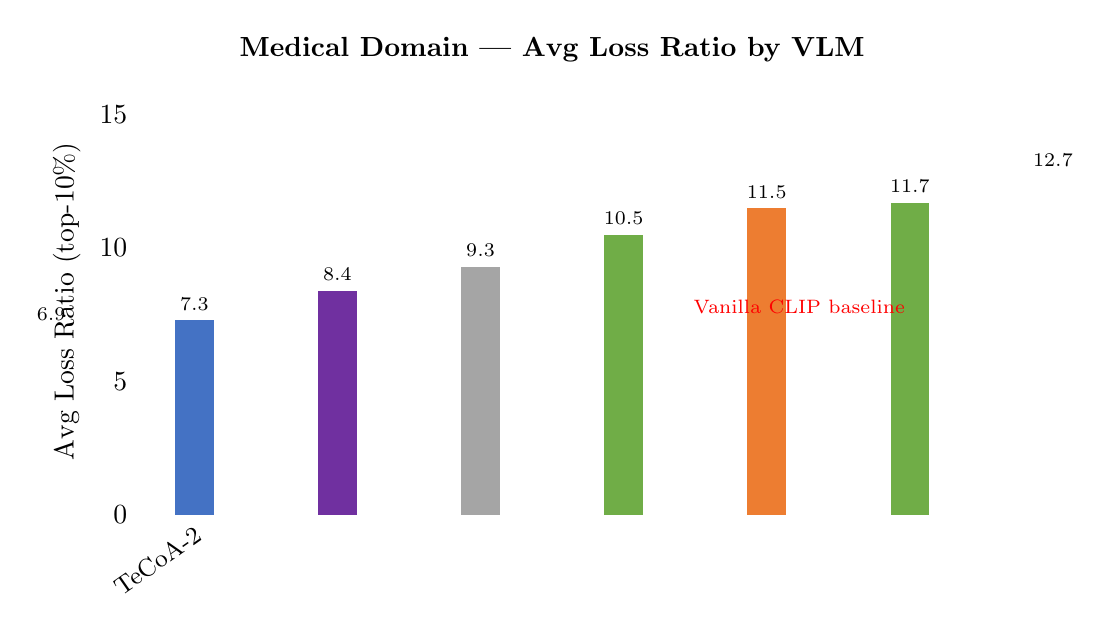
\begin{tikzpicture}
\begin{axis}[
    title={\textbf{Medical Domain --- Avg Loss Ratio by VLM}},
    ybar,
    bar width=14pt,
    width=\textwidth,
    height=7cm,
    ylabel={Avg Loss Ratio (top-10\%)},
    symbolic x coords={TeCoA-2, Vanilla CLIP, BiomedCLIP, TeCoA-4, FARE-2, SimCLIP-4, FARE-4, SimCLIP-2},
    xtick=data,
    x tick label style={rotate=35, anchor=east, font=\small},
    ymin=0, ymax=16,
    nodes near coords,
    nodes near coords style={font=\scriptsize},
    every node near coord/.append style={/pgf/number format/.cd, fixed, precision=1},
    legend style={at={(0.02,0.98)}, anchor=north west, font=\small},
    draw opacity=0,
]
\addplot[fill=tecoagray] coordinates {(TeCoA-2, 6.9)};
\addplot[fill=clipblue] coordinates {(Vanilla CLIP, 7.3)};
\addplot[fill=biomedpurple] coordinates {(BiomedCLIP, 8.4)};
\addplot[fill=tecoagray] coordinates {(TeCoA-4, 9.3)};
\addplot[fill=faregreen] coordinates {(FARE-2, 10.5)};
\addplot[fill=simcliporange] coordinates {(SimCLIP-4, 11.5)};
\addplot[fill=faregreen] coordinates {(FARE-4, 11.7)};
\addplot[fill=simcliporange] coordinates {(SimCLIP-2, 12.7)};
\draw[dashed, red, thick] (axis cs:Vanilla CLIP, 7.3) -- (axis cs:SimCLIP-2, 7.3);
\node[red, font=\scriptsize] at (axis cs:FARE-4, 7.8) {Vanilla CLIP baseline};
\end{axis}
\end{tikzpicture}
\caption{Most robust VLMs \textbf{increase} attack effectiveness on medical data. SimCLIP-2 is 74\% stronger than vanilla CLIP. Only TeCoA-2 is slightly below baseline.}
\end{figure}

\begin{figure}[h]
\centering
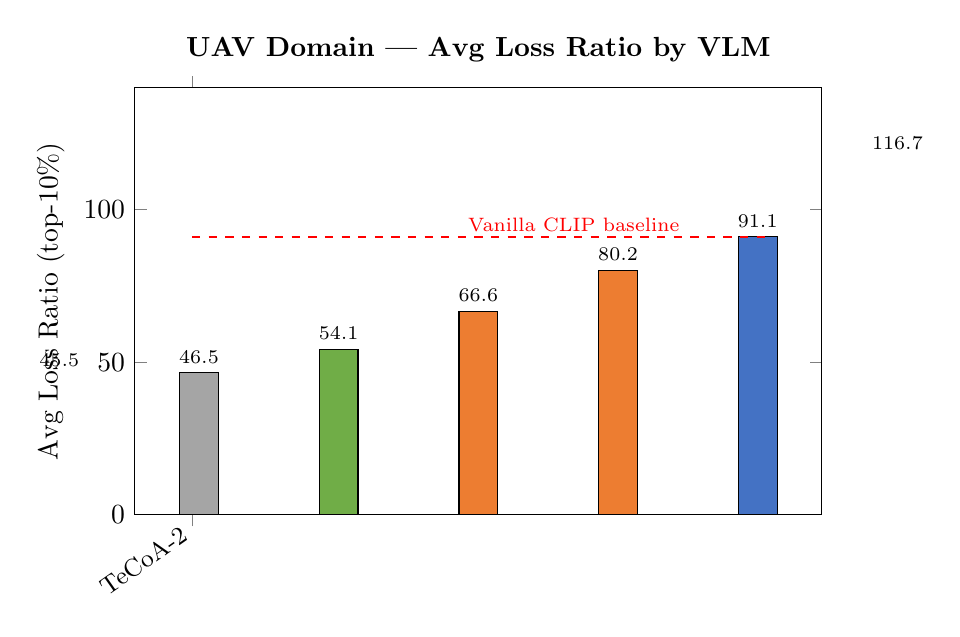
\begin{tikzpicture}
\begin{axis}[
    title={\textbf{UAV Domain --- Avg Loss Ratio by VLM}},
    ybar,
    bar width=14pt,
    width=0.85\textwidth,
    height=7cm,
    ylabel={Avg Loss Ratio (top-10\%)},
    symbolic x coords={TeCoA-2, TeCoA-4, FARE-4, SimCLIP-2, SimCLIP-4, Vanilla CLIP, FARE-2},
    xtick=data,
    x tick label style={rotate=35, anchor=east, font=\small},
    ymin=0, ymax=140,
    nodes near coords,
    nodes near coords style={font=\scriptsize},
    every node near coord/.append style={/pgf/number format/.cd, fixed, precision=1},
]
\addplot[fill=tecoagray] coordinates {(TeCoA-2, 45.5)};
\addplot[fill=tecoagray] coordinates {(TeCoA-4, 46.5)};
\addplot[fill=faregreen] coordinates {(FARE-4, 54.1)};
\addplot[fill=simcliporange] coordinates {(SimCLIP-2, 66.6)};
\addplot[fill=simcliporange] coordinates {(SimCLIP-4, 80.2)};
\addplot[fill=clipblue] coordinates {(Vanilla CLIP, 91.1)};
\addplot[fill=faregreen] coordinates {(FARE-2, 116.7)};
\draw[dashed, red, thick] (axis cs:TeCoA-2, 91.1) -- (axis cs:FARE-2, 91.1);
\node[red, font=\scriptsize] at (axis cs:SimCLIP-4, 95) {Vanilla CLIP baseline};
\end{axis}
\end{tikzpicture}
\caption{UAV results are mixed. FARE-2 actually \textbf{increases} attack effectiveness. TeCoA variants reduce it $\sim$50\% but loss ratios remain very high (45--47x).}
\end{figure}

\textbf{Why don't robust VLMs help?} SimCLIP/FARE defend CLIP against adversarial input perturbations. In Geminio, CLIP runs on the attacker's server processing clean images---no adversarial perturbations occur. Robust VLMs learn more semantically meaningful features, which inadvertently helps the attacker discriminate targets.

\clearpage
\section{DP-SGD Defense}

DP-SGD (Abadi et al., CCS 2016) clips gradient norms and adds calibrated Gaussian noise before sharing. It is the first defense that effectively stops Geminio.

\begin{figure}[h]
\centering
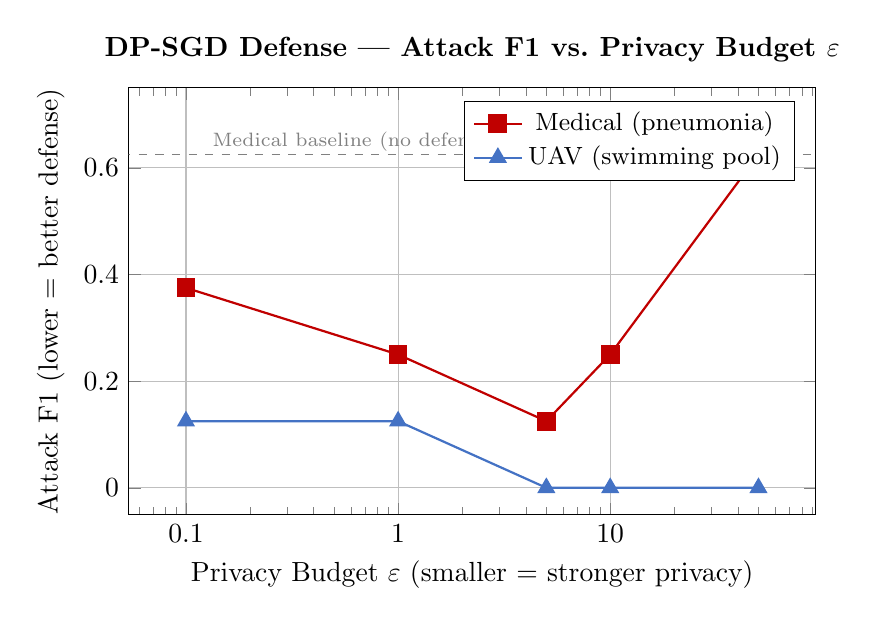
\begin{tikzpicture}
\begin{axis}[
    title={\textbf{DP-SGD Defense --- Attack F1 vs.\ Privacy Budget $\varepsilon$}},
    width=0.85\textwidth,
    height=7cm,
    xlabel={Privacy Budget $\varepsilon$ (smaller = stronger privacy)},
    ylabel={Attack F1 (lower = better defense)},
    xmode=log,
    log ticks with fixed point,
    ymin=-0.05, ymax=0.75,
    legend pos=north east,
    legend style={font=\small},
    grid=major,
    mark size=3pt,
]
\addplot[color=dpsgdred, mark=square*, thick] coordinates {
    (0.1, 0.375) (1.0, 0.250) (5.0, 0.125) (10.0, 0.250) (50.0, 0.625)
};
\addlegendentry{Medical (pneumonia)}

\addplot[color=clipblue, mark=triangle*, thick] coordinates {
    (0.1, 0.125) (1.0, 0.125) (5.0, 0.0) (10.0, 0.0) (50.0, 0.0)
};
\addlegendentry{UAV (swimming pool)}

\draw[dashed, gray] (axis cs:0.05, 0.625) -- (axis cs:100, 0.625);
\node[gray, font=\scriptsize, anchor=west] at (axis cs:0.12, 0.65) {Medical baseline (no defense)};
\end{axis}
\end{tikzpicture}
\caption{DP-SGD with gradient clipping (C=1.0) effectively stops Geminio. UAV targeting is completely eliminated even at $\varepsilon$=50 (minimal noise), because clipping alone disrupts the gradient amplification mechanism.}
\end{figure}

\begin{table}[h]
\centering
\caption{DP-SGD results at $\varepsilon$=5 (moderate privacy)}
\begin{tabular}{lcccc}
\toprule
\textbf{Domain} & \textbf{LPIPS} $\downarrow$ & \textbf{PSNR} $\uparrow$ & \textbf{Attack F1} & \textbf{vs.\ Baseline} \\
\midrule
Medical (no defense) & 1.019 & 10.86 & 0.625 & --- \\
Medical (DP-SGD $\varepsilon$=5) & 0.791 & 11.41 & \textbf{0.125} & \textbf{--80\%} \\
\midrule
UAV (no defense) & 0.679 & 12.88 & high & --- \\
UAV (DP-SGD $\varepsilon$=5) & 0.689 & 12.39 & \textbf{0.000} & \textbf{--100\%} \\
\bottomrule
\end{tabular}
\end{table}

\section{FedAvg Multi-Epoch Defense}

The Geminio paper noted that FedAvg with multiple local epochs weakens the attack. We tested this systematically.

\begin{figure}[h]
\centering
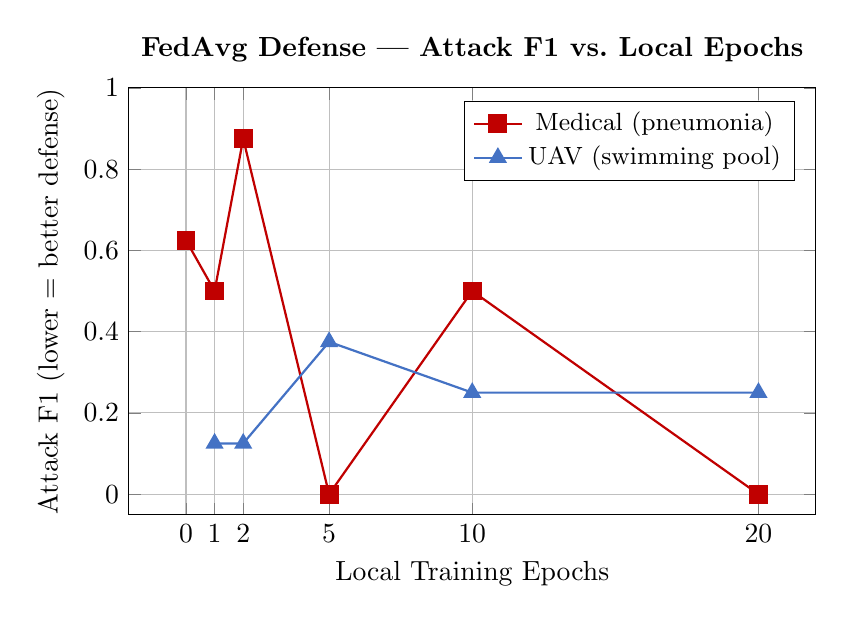
\begin{tikzpicture}
\begin{axis}[
    title={\textbf{FedAvg Defense --- Attack F1 vs.\ Local Epochs}},
    width=0.85\textwidth,
    height=7cm,
    xlabel={Local Training Epochs},
    ylabel={Attack F1 (lower = better defense)},
    ymin=-0.05, ymax=1.0,
    legend pos=north east,
    legend style={font=\small},
    grid=major,
    mark size=3pt,
    xtick={0,1,2,5,10,20},
]
\addplot[color=dpsgdred, mark=square*, thick] coordinates {
    (0, 0.625) (1, 0.500) (2, 0.875) (5, 0.000) (10, 0.500) (20, 0.000)
};
\addlegendentry{Medical (pneumonia)}

\addplot[color=clipblue, mark=triangle*, thick] coordinates {
    (1, 0.125) (2, 0.125) (5, 0.375) (10, 0.250) (20, 0.250)
};
\addlegendentry{UAV (swimming pool)}
\end{axis}
\end{tikzpicture}
\caption{FedAvg provides some defense but is \textbf{inconsistent}. Medical F1 is non-monotonic (0.000 at 5 epochs, 0.500 at 10). UAV stays low (0.125--0.375) but never reliably reaches 0.000.}
\end{figure}

\section{Complete Defense Comparison}

\begin{table}[h]
\centering
\caption{All defenses tested against Geminio}
\begin{tabular}{llcccc}
\toprule
\textbf{Defense} & \textbf{Level} & \textbf{Medical F1} & \textbf{UAV F1} & \textbf{Reliable?} & \textbf{Guarantee?} \\
\midrule
None (FedSGD) & --- & 0.625 & --- & --- & No \\
Gradient pruning 99\% & Gradient & inconsistent & inconsistent & No & No \\
Laplacian noise 1e-1 & Gradient & inconsistent & inconsistent & No & No \\
SimCLIP-4 & VLM & worse (+57\%) & --12\% & No & No \\
FARE-4 & VLM & worse (+61\%) & --41\% & No & No \\
FedAvg (5 epochs) & FL protocol & 0.000 & 0.375 & Partial & No \\
FedAvg (20 epochs) & FL protocol & 0.000 & 0.250 & Partial & No \\
\textbf{DP-SGD $\varepsilon$=5} & \textbf{Gradient} & \textbf{0.125} & \textbf{0.000} & \textbf{Yes} & \textbf{$(\varepsilon,\delta)$-DP} \\
\bottomrule
\end{tabular}
\end{table}

\end{document}
